\chapter{Literature Review}
\label{chap:Literature Review}

This chapter introduces several fundamental concepts pertaining to the research and provides a detailed background on the research topic, identifying current gaps and outlining potential areas for future research. 

\section{Introduction}
 The optimization of \acfp{BAS} has been a hot topic in past literature; however, the integration of semantic information within these systems has received very minimal research effort yet this integration has the potential to facilitate \textit{collective contextual reasoning} in building automation agents. This thesis defines collective contextual reasoning as the ability of building automation agents\footnote{For simplicity, this thesis will sometimes refer to building automation agents simply as \textit{"agents"}} to reason and make decisions based on the aggregated context of a building. This context can encompass heterogeneous parameters ranging from indoor to outdoor, such as the current state of the building, historical data, indoor comfort goals, weather conditions, and occupant behaviour. These parameters also have unknown latent dependencies that may be statistical in nature rather than deterministic. The previous chapter hypothesized that a holistic representation of building information is a prerequisite for building automation agents to infer hidden patterns in building information.

\section{The Need for Linked Data in the \ac{AEC/FM} industry}
The \ac{AEC/FM} industry is underpinned by a continuous flow and exchange of information during the design, construction and maintenance of the built environment \citep{Borrmann2010}. This information is usually fragmented and domain-specific due to the complex and departmental nature of the industry making reliable exchange and stakeholder collaboration a challenge \citep{Pauwels}. Furthermore, this fragmentation hinders the integration of expert knowledge among designers, contractors and facility managers diminishing their opportunity to optimally influence the design, construction and management of a built asset. \cite{MohdNawi2014} investigated the fragmentation issues of the \ac{AEC/FM} industry in detail and highlighted the resulting implications on project cost, schedule, dispute handling and unsustainable design-build routines. Autodesk's 2021 FMI report highlighted some surprising figures on how much data and time is wasted in the \ac{AEC/FM} industry i.e., 95.5\% of the construction data goes unused, 13\% of the construction professionals' working hours are spent looking for project information, and  30\% of \ac{AEC/FM} companies are using software that does not integrate with one another. \citep{Autodesk2021HarnessingConstruction}. Within the building automation context, most optimization strategies rely on heterogeneous building information that has been generated from various data islands and often exists in unrelated formats. When used in its raw unintegrated form, this information is ineffective and has a higher probability of being underutilized in many downstream building automation
tasks \citep{Borrmann2010,Pauwels}.  

\section{\ac{BIM}: A Prerequisite for Linked Building Data }
\label{BIM}   
The application of digital tools in building operations remains in its infancy, making it one of the biggest missed opportunities in building maintenance today \citep{Borrmann2010, Susan2023MindData}. Traditionally, at handover, facility managers receive piecemeal operational building information using \ac{PDF}, compact disc and other storage media. As a consequence, this information is often unstructured and semantically insufficient to support many downstream building operation tasks \citep{Zhang2015, Chen2018, Lu2019, Mason2019}. At the heart of the conversation on how this can be solved is \ac{BIM}, a workflow that effectively handles vast amounts of building information centrally within an intelligent three-dimensional model. The information management protocols offered by \ac{BIM} dramatically improve the coordination of \ac{FM} tasks, semantic enrichment of simulation models for training autonomous energy control algorithms \citep{Mason2019} and data-driven optimization of asset designs \citep{Lu2019b}. Furthermore, during operation, \ac{BIM} reduces the need for facility managers to manually enter asset data into \acp{CMSS}. This minimizes costly errors, clashes, data loss (see \autoref{Infloss}) and \ac{FM} blind spots, making it easier for facility managers to, locate, interact with, and report on space and asset data. 

\begin{figure}[!b]
	\centering
	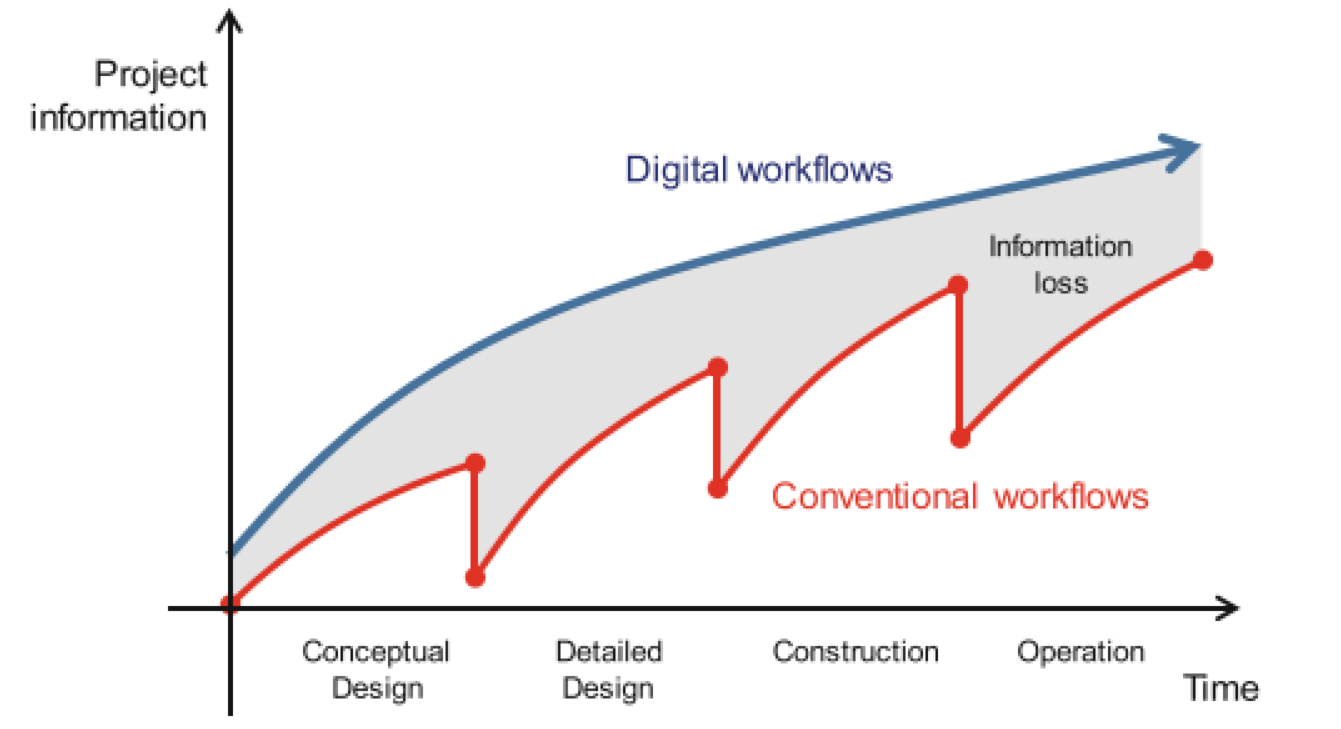
\includegraphics[width=0.65\textwidth]{figures/Informationloss}
	\caption{Information loss at various stages of the project lifecycle \citep{Borrmann2010}}
	\label{Infloss}
\end{figure}

 \begin{figure}[t]
	\centering
	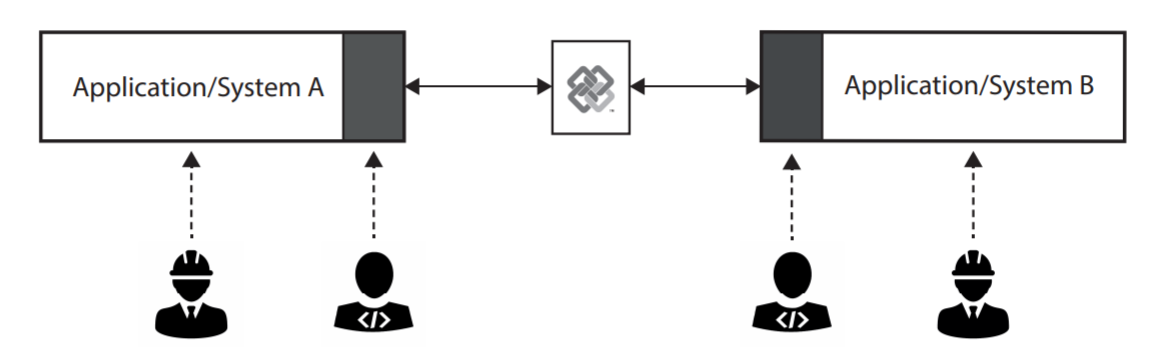
\includegraphics[width=0.7\textwidth]{figures/IFCworkflow}
	\caption{IFC exchange (which relies on end-users modelling expertise) between two BIM software via import-export routines implemented by software developers \citep{Zhang2019}.} 
	\label{IFCworkflow}
\end{figure}
For lossless data exchange and software interoperability, the \ac{BIM} ecosystem relies on \ac{IFC}, an open, vendor-neutral data exchange format developed by buildingSMART. \ac{IFC} is underpinned by technologies from EXPRESS \citep{ISO10303-11.2004}, an object-oriented data modelling language specifically designed for product modelling. A detailed description of its structure is provided by \cite{ISO10303-11.2004}, \cite{ISO10303-212016} and \cite{Pauwels2016}. Due to the comprehensive and generic nature of \ac{IFC}, it is extremely powerful in catering for different needs of presenting building information. However, this not only makes it a complex data model but also never entirely complete i.e. the generic flexibility gives undesired freedom for domain end users and application implementers by limiting the number of problem-specific constraints at the schema level. As a consequence, it is not uncommon for some software import-export routines (see \autoref{IFCworkflow}) to exercise data loss and errors during implementation \citep{Borrmann2010}. In fact \cite{Zhang2015} highlights how \ac{IFC}'s generality results in the lack of several problem-specific constraints and \cite{Msc2016} delineates how \ac{IFC} does not cover all data structures to meet the requirements of specific energy-management use cases. To satisfy specific data exchange scenarios such as energy simulations, acoustic performance and structural analysis, schema-level constraints are applied to \ac{IFC} using \acp{IDM} and \acp{MVD}. The constraints determine who provides which information when and to whom for a specific use case. When the \ac{IFC} schema was initially developed, its authors recognized the necessity for extensibility to accommodate the diverse use cases of the \ac{AEC/FM} industry \citep{Msc2016,Zhang2014} as discussed below. 

\begin{enumerate}
	\item 
	\ac{IFC} adopts a generic structure with only very few formalized constraints on the data model i.e. almost all attributes are \texttt{OPTIONAL} in the \ac{IFC} specification which means that hardly any attribute requires the mandatory provision of a value to be deemed valid at any stage of the lifecycle or exchange scenario. For specialized exchange use cases, \acp{MVD} are used to narrow down the wide scope of \ac{IFC} by determining which \texttt{OPTIONAL} attributes need to have values asserted to satisfy the requirements of that specific exchange use-case.     
	\item 
	Secondly, \ac{IFC} provides attribute extension mechanisms via \emph{property sets} and \emph{proxies}. As already mentioned, a syntactically correct \ac{IFC} instance might miss important attributes for a specific use-case, for example, the \texttt{IfcDoor} (an entity for modelling doors in \ac{IFC}) only has two mandatory attributes: \texttt{GlobalId} and \texttt{OwnerHistory}, \texttt{IfcWindow} only has \texttt{GlobalId} as a mandatory attribute. This information can only be used to identify and manage revisions of those object models. All the other information such as width, height, fire safety class, thermal performance and price is regarded as unnecessary for the syntactic validity of the underlying data model. This is where \emph{property sets} come in as an extension mechanism by dynamically creating new properties to supplement the already defined static attributes within the schema. The new individual properties are defined using \texttt{IfcPropertySingleValue} a subproperty of \texttt{IfcProperty}, and thereafter grouped into an \texttt{IfcPropertySet} which can be assigned to an object via \texttt{IfcRelDefinesByProperties}. In addition to property sets, is \texttt{IfcProxy}, a placeholder that permits dynamic definition of semantic information that is not yet defined by \ac{IFC} \citep{Borrmann2010}.

     \item 
     A further means of extending the IFC model is provided by externally referenced properties in libraries such as bSDD (buildingSMART Data Dictionary). Semantic web technologies (see \autoref{Semantic Web}) and Internet of Things (IoT) suggested in \cite{Debruyne2017, Jeroen2018, Pauwels, Zhang2015} are also steadily emerging as a means of providing more flexible semantic extension opportunities for the IFC schema. 
\end{enumerate}

The above overview is by no means exhaustive but highlights the most significant underlying concepts of \ac{IFC} data modelling using the EXPRESS language in an easy-to-understand fashion with the aim of putting the research problem into context. 

\subsubsection{Summary}
In attempting to address the shortcomings of heterogeneity and fragmentation within the \ac{AEC/FM} industry, \ac{BIM} emerged as a model-centric approach for propagating and handling information holistically along the building lifecycle. Of course with the advent of \ac{BIM}, a standardized way of representing and exchanging building information emerged as an open and vendor-neutral standard, \ac{IFC} developed by buildingSMART. Since the first version, \ac{IFC} 1.0 in 1997 to the current IFC 4, it has matured extensively into a popular data model implemented by many \ac{AEC/FM} software. This maturity has no wonder caught the attention of international bodies thus making it a fully operational ISO standard \citep{ISO16739:202424} and it has become a mandatory data exchange format during construction tendering in some countries \citep{AEC-UK2012}. To cater for a wide range of use cases, the \ac{IFC} data model is very generic with only a few internally defined constraints providing users with the flexibility of representing building information in a variety of ways depending on the use case. This, however, results in a very large and complex data model for software implementers. To this effect, buildingSMART further developed \acp{MVD} which reduces this complexity by explicitly specifying which parts of the data model need to be implemented for a specific data exchange routine. This is the basis for buildingSMART's certification process of \ac{BIM} software. It is evident that the \ac{AEC/FM} industry is responding to its ever-increasing complexity by embracing linked and interoperable semi-automated workflows however, \cite{Pauwels2016, Pauwels2017, Pauwels} highlights that \ac{IFC} considerably improves \emph{but does not} solve information interoperability within the \ac{AEC/FM} industry because of the lack of formal explicit and context-aware semantics in EXPRESS \citep{Barbau2012} therefore making domain-agnostic semantic extensions for the underlying \ac{IFC} data model a necessity.  

\section{Extending \ac{BIM} with Semantic Web Technologies}
\label{Semantic Web}
The ecosystem of current BIM software is closed and optimized only for the \ac{AEC/FM} industry making it difficult for other disciplines to become part of the BIM story \citep{Jeroen2018}. Considering that optimization problems within the industry are reliant on several domain experts who generate a lot of heterogeneous information, having explicit interdisciplinary collaboration is of paramount importance. Unlike domain-specific \ac{BIM} \citep{Pauwels}, a methodology that allows various disciplines to interlink their knowledge on a data level is already existent with principles based on the classic 
\textit{\ac{WWW}} \citep{Berners-Lee2001a, Berners-Lee2001}. The common framework that allows such heterogeneous knowledge integration, sharing and re-use is called the \textit{Semantic Web}. Its aim is to harmonize semantic ambiguity and discrepancies in heterogeneous data schemata by adding standardized machine-readable semantics \citep{Barbau2012} using the \ac{RDF} data model. For a building energy optimization use case, this means that non-geometrical heterogeneous data from other domains can be used to supplement an energy analysis building model with valuable attributes. Homogeneity of this nature cannot be achieved using the \ac{BIM}'s native \ac{IFC}-EXPRESS schema therefore necessitating schema translations into open and extensible data structures using \acf{SWT} such as \ac{RDF} \citep{Pan2004, Pauwels2010, Yang2006}. 

The \ac{RDF} data model \citep{Manola2014} is in parallel with object-oriented modelling approaches in \ac{IFC} where notions of \emph{entities/classes} related by \emph{associations} are respectively represented in \ac{RDF} using \emph{concepts} related with \emph{properties} \citep{Pauwels2016}. Anything described in the semantic web context is called a \emph{resource} and is identified via a \ac{URI}  \citep{Studer2007}. \ac{RDF} provides a way of semantically describing these resources by making simple statements about them. These statements are called \emph{triples} and syntactically take the \texttt{subject-predicate-object} format \citep{Manola2014} as shown in \autoref{RDF triple}. Multiple statements about the same resource increase its semantic meaning and richness as shown in \autoref{RDF triple} and \autoref{RDF graph} to form a \textit{knowledge graph}. \acp{URI} can be very long making triples less human-readable and may contain
prohibited characters for resource labeling. Therefore, \acp{QName} are often adopted as abbreviations to \acp{URI}. A \ac{QName} has two parts; a namespace and
an identifier in the form \texttt{namespace:identifier}. To store \ac{RDF}
triples in a compact web-publishable form, several serialization formats can be used i.e., Turtle \citep{Beckett2011}, N3 JavaScript \citep{Berners-Lee2011}, RDF/XML \citep{Beckett2014} and JSON-LD \citep{Kellogg2019}. When several resources related to a specific domain are organized together using formal logics \citep{Baader2003, Hitzler2012, W3COWLWorkingGroup2012}, they form an ontology or vocabulary. \ac{RDF} alone is not expressive enough to describe ontologies, but together with \ac{RDFS} and \ac{OWL}, it is possible. The complexity and vastness of semantic web models necessitate a methodology for searching, filtering out and validating the information from them. \ac{SPARQL} plays this role both locally and when dealing with federated resources \citep{Harris2013, W3CSPARQLWorkingGroup2013}.
\begin{figure}[!t]
	\centering
	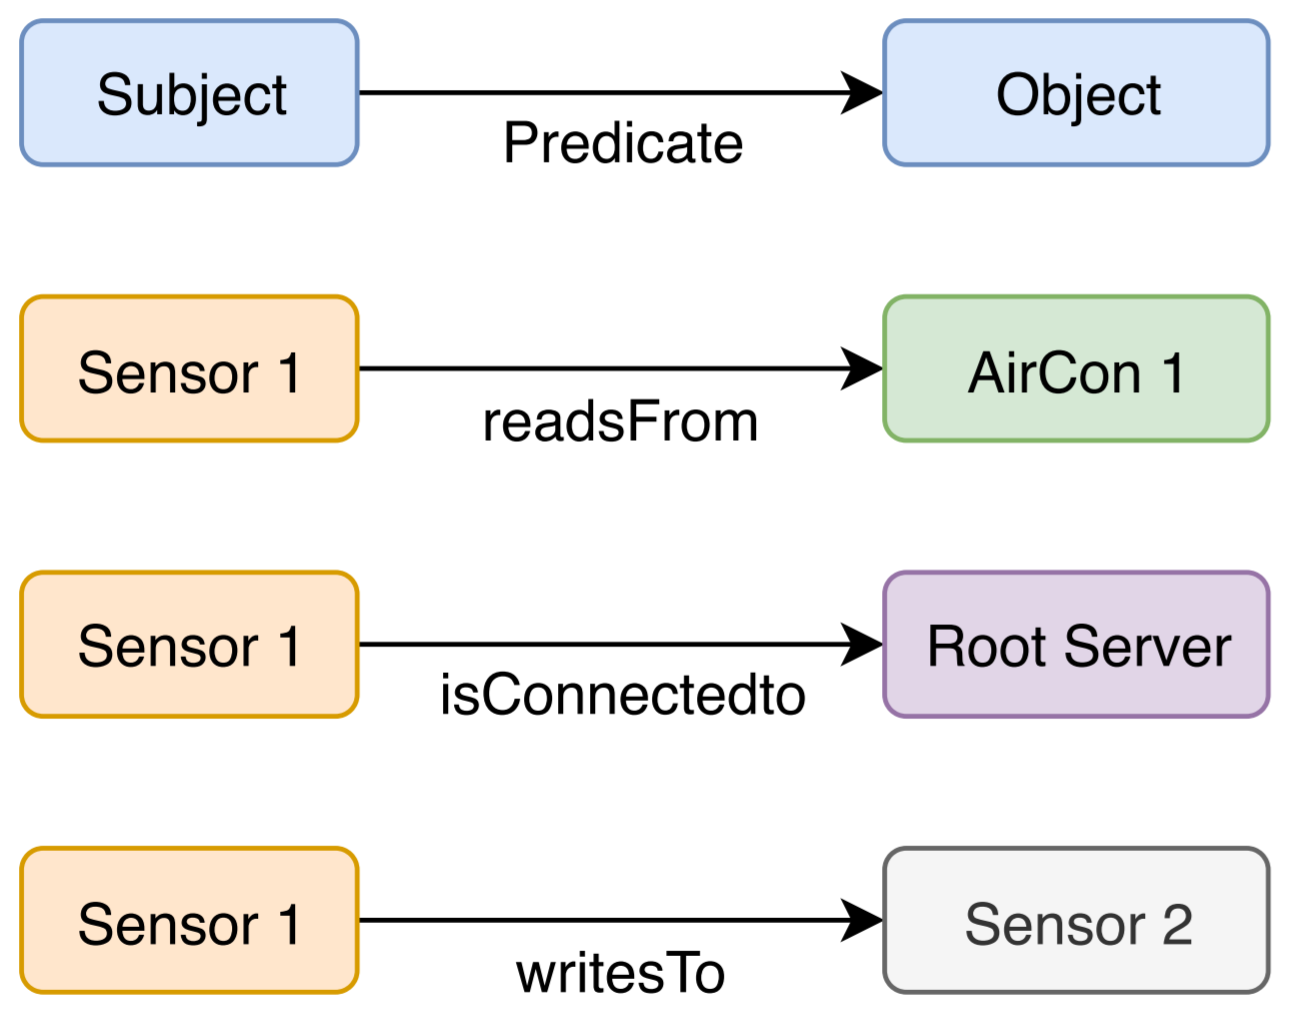
\includegraphics[width=0.3\textwidth]{figures/RDFtriple}
	\caption{RDF triples in the form \emph{subject-predicate-object}. The arrows imply directionality of the relationship.} 
	\label{RDF triple}
\end{figure}

\begin{figure}[!t]
	\centering
	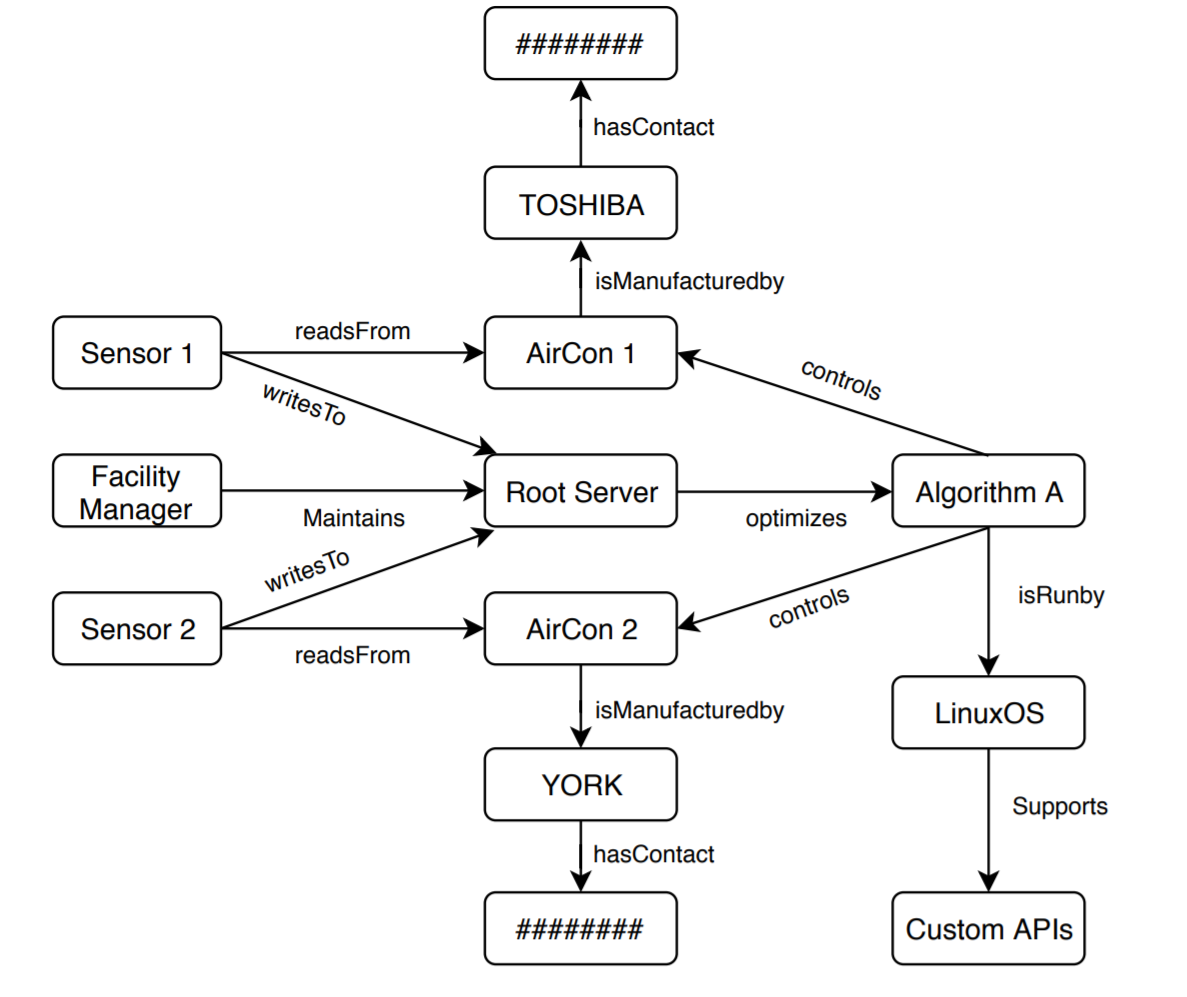
\includegraphics[width=0.5\textwidth]{figures/RDFgraph}
	\caption{An example of an RDF graph (combination of triples) describing some information about sensors in a building connected to different air conditioning units and managed by a root server.} 
	\label{RDF graph}
\end{figure}


\begin{lstlisting}[captionpos=b, caption=A basic SPARQL query retrieving AC units whose sensor value is above a certain set threshold. No specific query modifiers have been defined, label=lst:sparql,
basicstyle=\ttfamily\small,frame=single]
PREFIX erlo: <http://unmcsharepoint/KevinLM/energyRLO/erlo.ttl#>
PREFIX rdf: <http://www.w3.org/1999/02/22-rdf-syntax-ns#>
PREFIX rdfs: <http://www.w3.org/2000/01/rdf-schema#>
FROM <http://unmcsharepoint/KevinLM/energyRLO/erlo.ttl>
SELECT ?ACunits ?sensor ?value
WHERE {
?erlo:ACunits rdf:type ?erlo:BuildingEquipment .
?erlo:erlo:Sensor erlo:readsFrom ?erlo:ACunits .
?erlo:Sensor erlo:hasValue ?erlo:AboveThresholdSensorValue .
} 
\end{lstlisting} 

Several early efforts to embrace \ac{SWT} within the industry emerged with reliance on project-specific ontologies that were hard to re-use or extend formally to other domains because of the different vocabularies and taxonomies employed. Some of these works include the e-COGNOS project from which the e-COGNOS ontology emerged \citep{Wetherill2002}, the inteliGrid project ontology for sharing semantics between applications \citep{Dolenc2007}, \cite{Yang2006}'s proposal of an early prototype to support inter-operability of \acp{BIM} and project data, \cite{Elghamrawy2008,Elghamrawy2010}'s ontologically driven model that supports management of and learning from construction problems by holistically integrating project data. Other notable research in this area can be found in \cite{Abdul-Ghafour2007, Le2016, Pauwels2010, Scherer2012, Shah2011} and \cite{Venugopal2015}.

In a push for standardization, a recommendable and reusable \ac{OWL} translation of \ac{IFC} (ifcOWL) was proposed by \cite{Pauwels2016} which was later agreed upon by the Linked Data Working Group (LDWG) \citep{W3C2014}. Prior to this however, several efforts to convert \ac{IFC} to \ac{RDF} were made by \cite{Agostinho2007, Beetz2005, Krima2009, Pauwels2015a, Schevers2005} and \cite{Zhao2008} whose proposals formed the basis for \cite{Pauwels2016}'s work. The ifcOWL ontology has further been modified by \cite{Pauwels2017} for a better representation of geometric data.  \cite{Terkaj2015} proposed an extension to ifcOWL in which \texttt{EXPRESS WHERE} rules were translated to OWL and included in the ifcOWL ontology. In addition, \cite{Gomez-Romero2015} proposed a fuzzy logic-based extension to the ifcOWL ontology that provides support for imprecise knowledge representation and retrieval which is characteristic of ontologies. 

The ifcOWL ontology is very large as it encapsulates the entire IFC schema and without a doubt, can often prove to be redundant in several use cases or even hard to query. To this effect, W3C's \ac{LBDCG} \citep{W3C2014} has progressively developed simpler, modular and extensible ontologies with intent to cover the IFC schema in smaller and more manageable modules, with \ac{BOT} \citep{Rasmussen2017a, Rasmussen2017, Rasmussen2019} proving to be the most reliable baseline module. \ac{BOT} serves as the key ontology for capturing the building topology (see \autoref{BOTZones}) which is extensible to other domain ontologies like the building device automation domain \citep{Bonino2018, Schneider2017, Villalon2017}, sensor domain \citep{Haller2017}, geospatial domain \citep{McGlinn2017}, and \ac{FM} domains.

\begin{figure}[t]
	\centering
	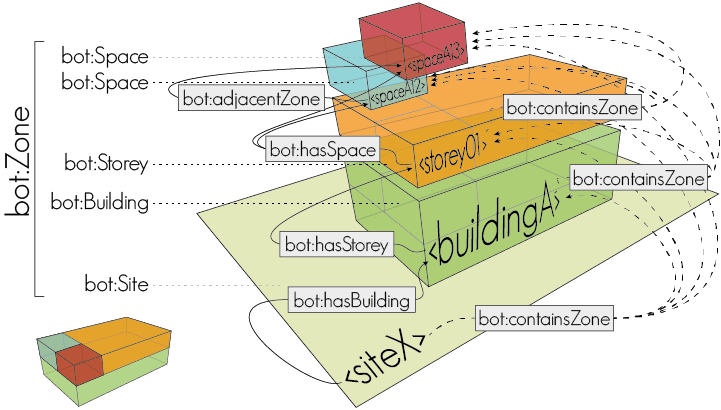
\includegraphics[width=0.6\textwidth]{figures/zones.png}
	\caption{Zone connectivity as defined in the \ac{BOT} ontology \citep{Rasmussen2017}.} 
	\label{BOTZones}
\end{figure}

Specific to building automation, several research efforts have emerged to embrace semantic web approaches in solving energy optimization problems. For instance, \cite{Curry2012} combined Linked Data with scenario modelling to support inter-operability during optimization of building performance. \cite{Msc2016} analysed 33 EU projects that utilized \ac{BIM}-based energy management plus their data requirements in order to identify those that can benefit from open linked data structures. \cite{Anzaldi2014} proposed a holistic knowledge-based approach for intelligent building energy management using a combination of ontologies, algorithms and simulations.  \cite{Radulovic2015} even went ahead to present a set of best practices and guidelines for generating and publishing Linked Data with \acp{BIM} in the context of energy consumption in buildings. \cite{Corry2015} and \cite{Scherer2012} developed a performance assessment ontology that structures heterogeneous building data into semantically enriched information which can support the energy management of buildings. A unified energy representation for smart cities via the DogOnt ontology was proposed by \cite{Bonino2018} by integrating several sub-domains of energy representation namely; electrical, thermal and city-level energy profiles. \cite{Dibley2011} and \cite{Dibley2012} coupled a multi-agent system with an ontology, 'OntoFM' to support real-time monitoring of building sensors in an automated and holistic way. Their work inherited principles from a building ontology based on \ac{IFC}, a sensors ontology (OntoSensor) \citep{Russomanno2005} and a general purpose ontology SUMO (Suggested Upper Merged Ontology) \citep{Niles2001} which captures domain-independent concepts. To support interoperability and exchange of data between building energy simulation tools, `SimModel', an XML-based data model, was proposed by \cite{Donnell2011}.  \cite{Pauwels2014,Pauwels2014a} then went ahead to avail this model as \ac{RDF} graphs which can be combined with other \ac{RDF} data. \cite{Tah2011} developed an ontology to represent information about photovoltaic systems. \cite{Reinisch2011} and \cite{Kofler2012} proposed a comprehensive 'ThinkHome system' that relies on an extensive ontological knowledge base to store all information needed to fulfil goals of energy efficiency and user comfort in future smart homes. This multi-agent system interacts with the knowledge base via \ac{SPARQL} queries and \ac{DL} inference to autonomously control a smart home. Much of the ThinkHome Ontology is inspired by DomoML-env \citep{Sommaruga2005}, an ontology for human-home interaction aiming to connect household appliances and share information about their usage. The aforementioned ontologies can also be combined with a set of \ac{SWRL} rules that automatically apply energy management strategies through inference with the knowledge base \cite{Rossello-Busquet2011}. Specifically, these rules enable the inference engine to infer if any anomalous activities are occurring (e.g. `air conditioners' that are `working' AND `windows' that are `open'). A \ac{SPARQL} endpoint can even be put on top of this rule engine so that the user only has to query for the results of the rules. Other systems utilizing the same \ac{SWRL} approach to managing smart home appliances have been proposed by \cite{Ricquebourg2007} and \cite{Tomic2010}.

Another growing trend in the building energy domain is the use \ac{DRL} as a means to automate energy optimization processes through \emph{sequential decision making} \citep{LeCun2015,Sutton1988}. Very little work has been done to assess how well \ac{DRL} models perform when fused with \ac{RDF}-based building datasets.


\section{Augmenting \acp{BIM-KG} with \acf{ML}}
\label{Knowledge graphs with DRL}

Just like the \ac{AEC/FM} domain has evolved to embrace \acp{SWT}, \ac{ML} is recognizing the growing need to learn from disparate data sources. \cite{Wilcke2017} discusses the current shift in data science from manual feature engineering to utilizing raw data, emphasizing the need for models that can directly consume and learn from diverse types of information scattered across different domains. To achieve this, a data model capable of expressing heterogeneous knowledge naturally in diverse domains is required, and \cite{Wilcke2017} argues that a knowledge graph is a suitable candidate. For a specific \ac{ML} task, it is possible to have good data sources with the right information but, without making it ripe for consumption i.e., exposing the inherent relationships in the data and adding useful semantics to enhance its context, it is just a boring mountain of unintelligent information that \ac{ML} models will struggle with to deduce informed decisions. Furthermore, by being able to model incomplete knowledge using the \ac{OWA} \citep{Berners-Lee2001,Berners-Lee2001a}, knowledge graphs are well suited for modelling real-world data without being concerned how the incompleteness should be dealt with, as is the case with many traditional \ac{ML} methods that need to employ complex and computationally expensive data imputation techniques when faced with missing or incomplete data \citep{Cunningham2007, Sterne2009, Priya2015}. A knowledge graph can use its intrinsic relationships to gracefully accommodate missing information by providing \ac{ML} models the ability to reason over the graph structure and infer new connections based on known relationships. This means that a knowledge graph has the flexibility of representing implied facts from explicitly declared knowledge without the need to include the implied triples in the graph. This allows knowledge graphs to achieve high levels of semantic expressivity without being redundant, overly large and complex at the expense of representing many facts.

\begin{figure}[t]
	\centering
	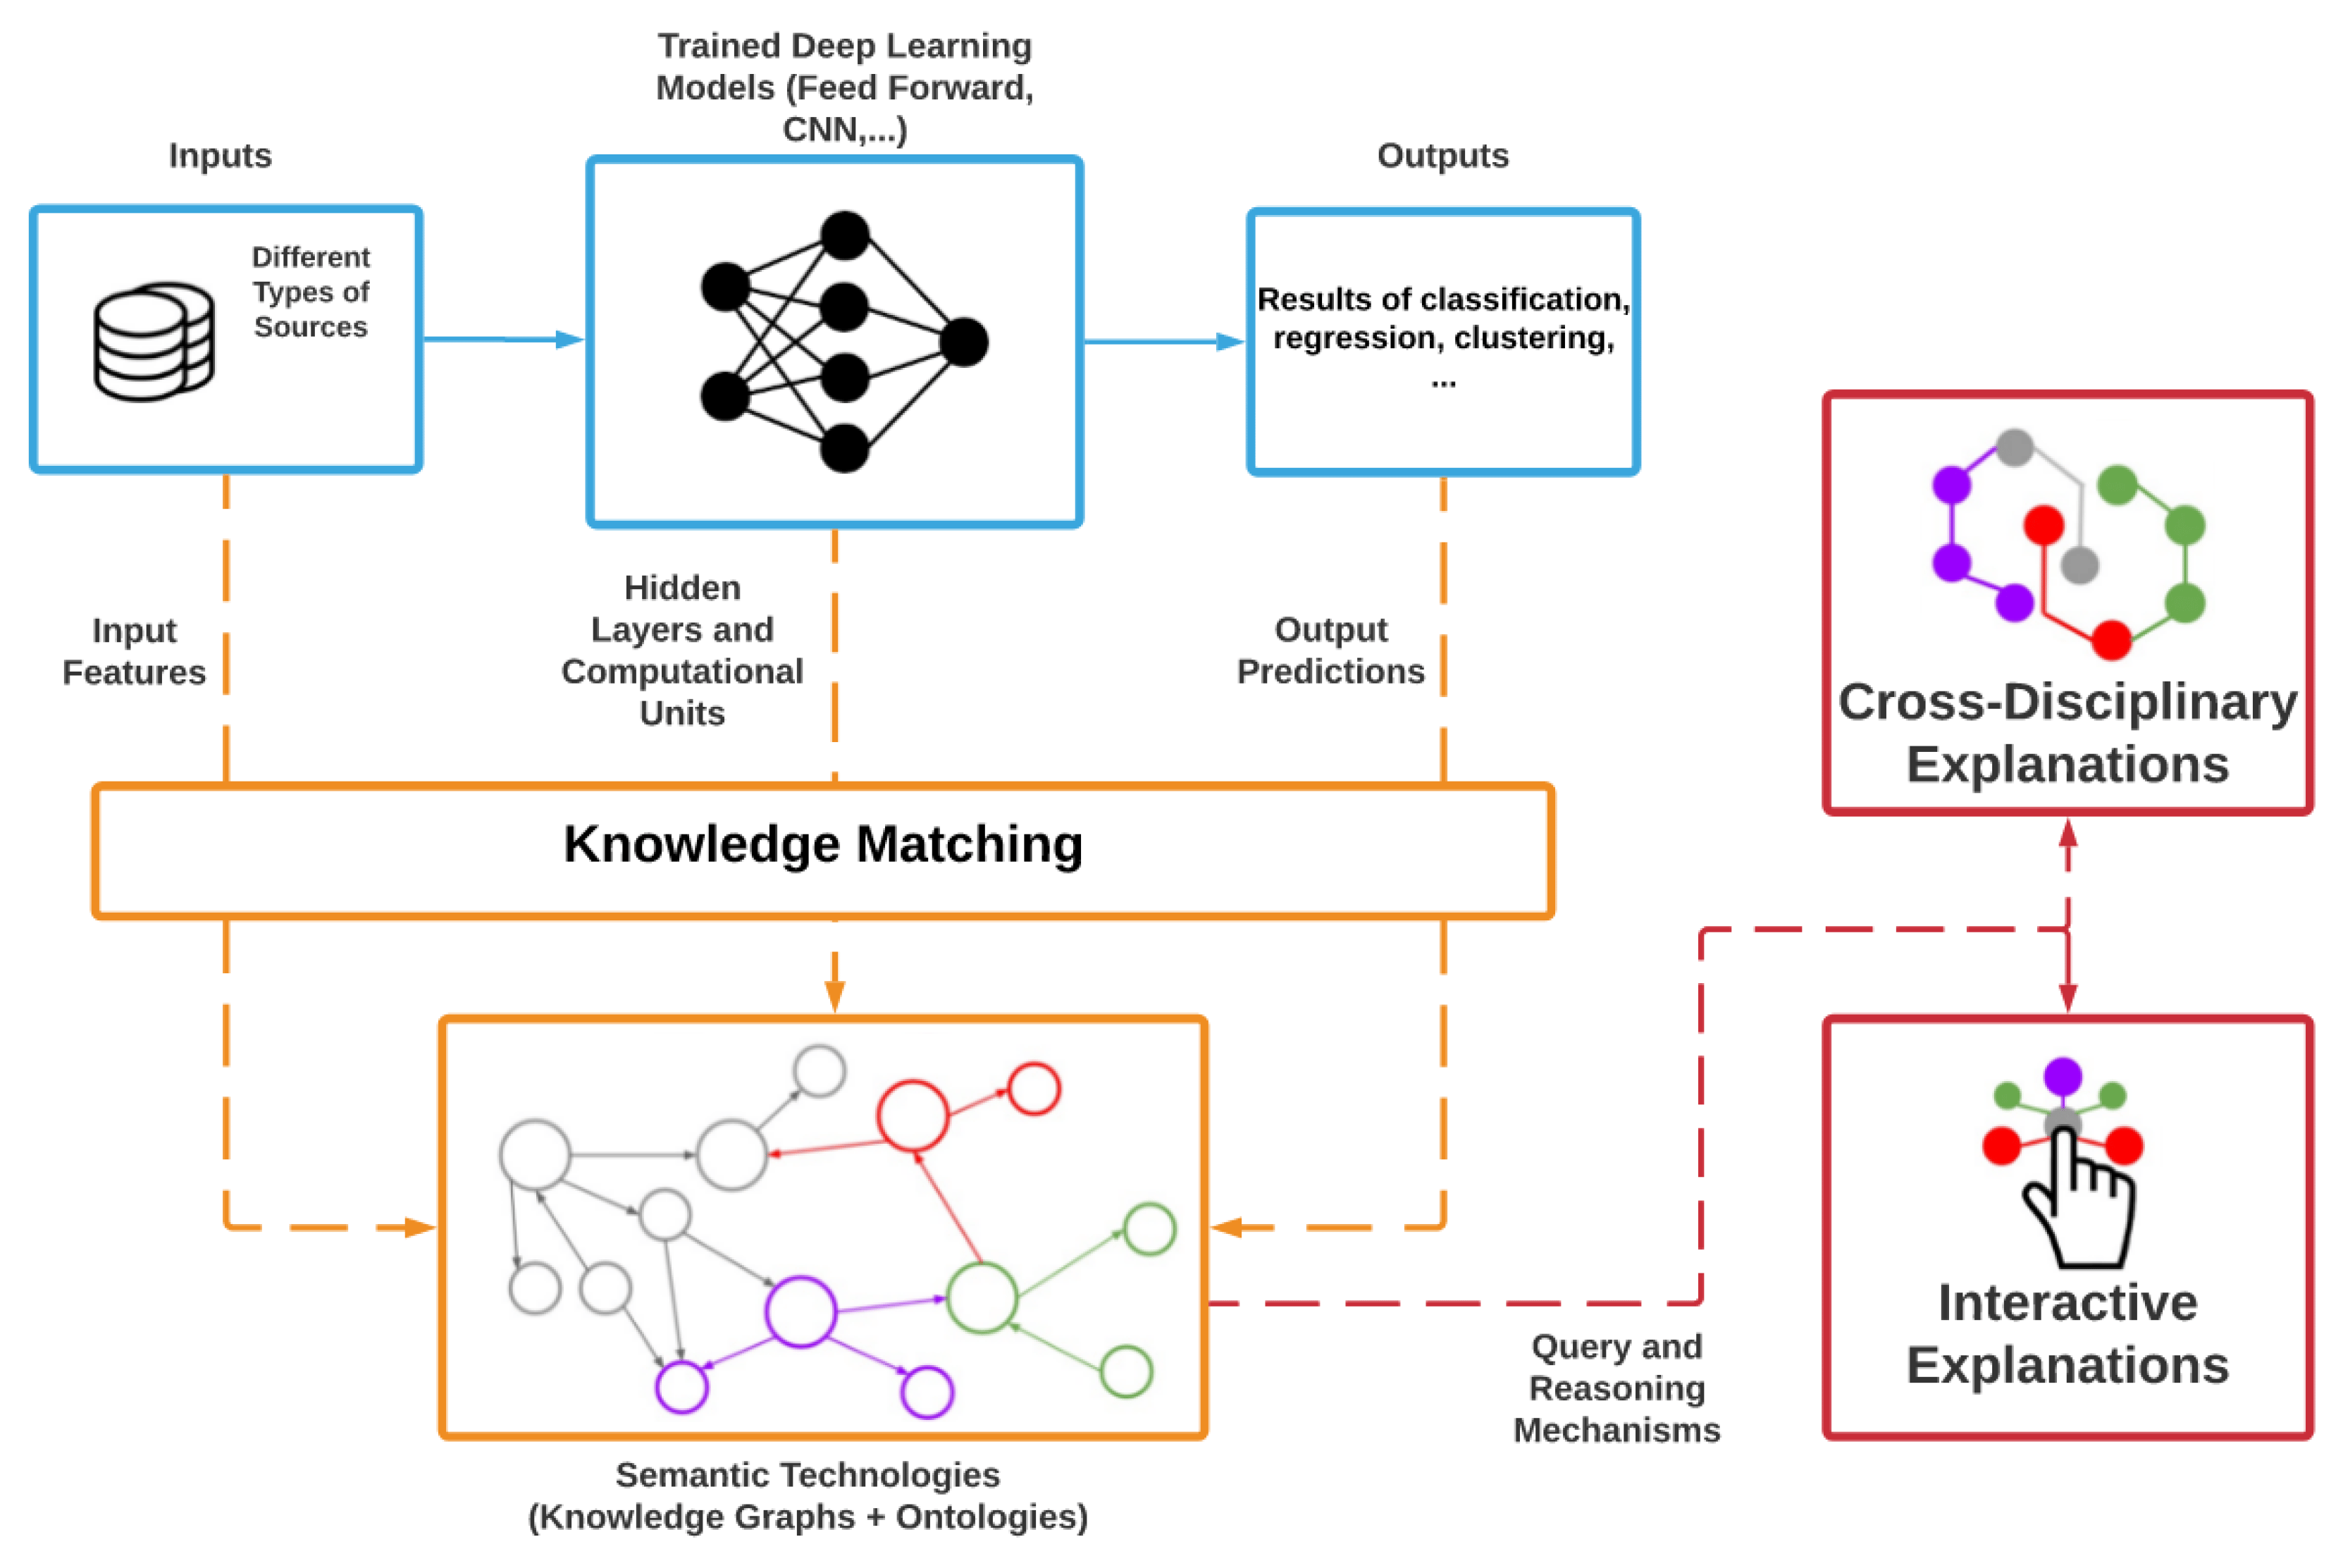
\includegraphics[width=1.0\textwidth]{DL-KG.png}
	\caption{Schematic representation of a system that integrates \acp{SWT} into deep learning \citep{Futia2020OnResearch}.} 
	\label{DL-KL}
\end{figure}

The emergence of deep learning models has paved the way for workflows that deal with extremely large raw data to automatically learn relevant features without the need for too much pre-processing, however, most present models are domain specific: tailored to image \citep{Cun1990, Krizhevsky, Le2013, Lowe1999}, sound or language \citep{Graves2013, Nguyen2015}, and when faced with heterogeneous knowledge, they struggle and often have to rely on manual pre-processing, a step at which a lot of vital learning information (hidden relationships) can be lost \citep{Wilcke2017}. Recently, the \ac{ML} community has taken a keen interest in making the knowledge graph part of the learning process (see \autoref{DL-KL} for a high-level schematic of such learning). Some methods still require a great deal of pre-processing while while others try to work with knowledge graphs more naturally. The former first translates knowledge graphs into feature vectors, which are a more manageable form to many existing learning methods. An example is substructure counting graph kernels \citep{Losch2012}, a type of algorithm designed to create feature vectors for individual nodes in a knowledge graph. They do this by tallying different types of substructures found near each node in a fashion similar to K-Nearest Neighbour methods in \cite{Cunningham2007}. A drawback of these substructure counting methods is that the size of the feature vector grows with the size of the data which led to a proposal of RDF2Vec by \cite{Ristoski2016} to handle large graphs more efficiently. More natural workflows of dealing with knowledge graphs include representing triples as a third-order tensor and adopting tensor decomposition methods for collective learning \citep{Kolda2009TensorApplications, Nickel2013TensorLearning}. \ac{GCN} \citep{Kipf2016} can also be used to model and learn from relational data more naturally as described by \cite{Schlichtkrull2017}. \cite{Nickel2016} provides a very comprehensive review on the use \ac{SRL} on knowledge graphs. \ac{SRL} uses probabilistic models to capture the uncertainty and dependency structure of entities in a knowledge graph. Traditional \ac{SRL} methods, such as Inductive Logic Programming \citep{Muggleton1994InductiveMethods}, Rule mining \citep{Volker2011StatisticalInduction}, and graphical models \cite{Wainwright2008GraphicalInference}, have been widely used for learning from graphs. However, these methods suffer from scalability issues as the number of statistical dependencies increase. They also require extensive prior knowledge about the learning task at hand which can be very computationally expensive to infer if it is not available. One of the most difficult aspects of knowledge graphs is the lack of spatial locality, which implies that the graph's structure cannot be effectively represented as a fixed grid. Furthermore, the graph isomorphism problem, which refers to the difficulty of determining whether two graphs are structurally identical, adds to the difficulty of learning from knowledge graphs. This is a known problem that is neither NP-complete nor solvable in polynomial time, rendering it computationally difficult for traditional \ac{SRL} methods that rely on manual feature engineering. Also, because knowledge graphs can represent multimodal data such as text, numbers, and timestamps, traditional \ac{SRL} approaches with limited expressivity struggle to model and learn from such complex representations. To overcome these challenges, \acf{KRL} methods have gained a lot of traction. These approaches aim to learn embeddings for nodes and edges within a knowledge graph without the need for manual feature engineering. Embeddings capture the essential characteristics and relationships of the graph's entities using dense vector representations. These vectors are learned in such a way that similar nodes or edges in the graph have similar embeddings. The key idea behind embeddings is to transform the knowledge graph, which is often complex and high-dimensional, into a lower-dimensional space where latent patterns can be discovered, more easily analyzed and utilized in downstream tasks such as link prediction, node classification, and community detection. An important aspect of embedding techniques is the notion of score functions. These are mathematical formulations that assess how likely a triple is to be true based on the learnt embeddings, with a larger score typically implying a more plausible triple.  For a triple \((h, r, t)\), the score function \(f(\mathbf{h}, \mathbf{r}, \mathbf{t}) \) maps it to a scalar value \(s \in \mathbb{R}\) that reflects the plausibility of the triple being true. Each entity \(h\) and \(t\) and the relation \(r\) are represented as vectors in a \(d\)-dimensional continuous vector space, with embeddings \(\mathbf{h}, \mathbf{t}, \mathbf{r} \in \mathbb{R}^d\).

Certain application fields such as social network analysis \citep{Xu2021UnderstandingApplications}, drug discovery in bio-informatics \citep{MacLean2021KnowledgeDiscovery}, and fraud detection in e-commerce \citep{Shen2021FinancialDetection} often deal with immensely interwoven and complex dataset structures. \ac{KRL} is one aspect of \ac{ML} that has made significant strides in understanding the idiosyncracies of these datasets, however the same cannot be said for its application in the \ac{AEC/FM} domain, yet it exhibits similarly intricate datasets. To the best of the author's knowledge, no work has been done to comparatively assess the performance of \ac{KRL} models when applied to \acp{BIM-KG}. To enhance reproducibility, trust and fair comparison of newly developed models against well-established baseline approaches, it is important to report model architectures, training steps, hyperparameters and dataset split mechanisms alongside any performance metrics. 

\section{An Intuitive Mathematical Perspective to Learning from \acp{BIM-KG}}
\label{learning in LBD domains}

For this thesis, a mathematical explanation from both set theory and first-order logic is not only deemed appropriate to define relational data but also highlights the relevance of exploiting the intrinsic relational structure of \acp{BIM-KG} in downstream building automation tasks. Relations, in general, define connections between entities, such as whether two rooms have a wall that connects them, whether a person has a specific indoor comfort preference, or whether a sensor is found in a particular space of a building. More precisely, in the domain of set theory and first-order logic, an \textbf{\textit{n-}}ary relation $\mathcal{R}$ over sets $\mathcal{A\textsubscript{1}}$, $\cdot$ $\cdot$ $\cdot$, $\mathcal{A\textsubscript{n}}$ is defined as a set of ordered \textbf{\textit{n-}}tuples\footnote{A tuple is useful for aggregating data that is needed to be considered as a single unit.} $\langle$\textit{a\textsubscript{1}, $\cdot$ $\cdot$ $\cdot$, a\textsubscript{n}}$\rangle$ where \textit{a\textsubscript{i}} is an element of $\mathcal{A\textsubscript{i}}$ $\forall$ \textit{i}, \textit{1}$\leqslant$ \textit{i} $\leqslant$ \textit{n}. More intuitively, an \textbf{\textit{n-}}ary relation $\mathcal{R}$ is a subset of the Cartesian product of \textit{n} sets \citep{Halmos1974NaiveTheory} (Chapter 7) $\mathcal{A\textsubscript{1}}$, $\cdot$ $\cdot$ $\cdot$, $\mathcal{A\textsubscript{n}}$, formally expressed as:
\begin{equation}
    \mathcal{R} \subseteq \mathcal{A\textsubscript{1}} \times \cdot \cdot \cdot \times \mathcal{A\textsubscript{n}}
\end{equation}
The relation $\mathcal{R}$ is interpreted as the set of all \textit{existing} relationships, while the Cartesian product is interpreted as the set of all \textit{possible} relationships over the entities in the domains $\mathcal{A\textsubscript{1}}$, $\cdot$ $\cdot$ $\cdot$, $\mathcal{A\textsubscript{n}}$. A single \textbf{\textit{n-}}tuple $\langle$\textit{a\textsubscript{1}, $\cdot$ $\cdot$ $\cdot$,a\textsubscript{n}}$\rangle$ therefore represents a possible relationship between the entities \textit{a\textsubscript{1}, $\cdot$ $\cdot$ $\cdot$,a\textsubscript{n}}, which we simply denote by   $\mathcal{R}$$\langle$\textit{a\textsubscript{1}, $\cdot$ $\cdot$ $\cdot$,a\textsubscript{n}}$\rangle$. With this background, it is evident that the RDF data modelling structure adopts \textit{binary or dyadic relations} of the form:
\begin{equation}
    \mathcal{R} \subseteq \mathcal{A\textsubscript{1}} \times \mathcal{A\textsubscript{2}}
\end{equation}
There are situations in \ac{RDF} which require the modelling of \textbf{\textit{n-}}ary relations involving more than two sets of entities. These can be handled efficiently using blank nodes that intrinsically force back a dyadic relational structure. Assuming that \textit{entities} of a particular type, for instance, sensors are encapsulated within a set, $\mathcal{E\textsubscript{m}}$. Similarly, let a set $\mathcal{L\textsubscript{n}}$ hold possible \textit{literals} values associated with the datatype property of an entity, for instance, a sensor reading, last calibration date of a sensor, U-value of a window glass. Then, any relation $\mathcal{R}$ $\subseteq$ $\mathcal{E\textsubscript{i}}$ $\times$ $\mathcal{E\textsubscript{j}}$ is an object property while $\mathcal{R}$ $\subseteq$ $\mathcal{E\textsubscript{i}}$ $\times$ $\mathcal{L\textsubscript{j}}$ is a datatype property. Typical \ac{NRML} settings utilize data that is literal valued and spanning over a single type of entity i.e. consisting relations that take the form $\mathcal{E}$ $\times$ $\mathcal{L\textsubscript{j}}$, with $\mathcal{E}$ denoting the set of all entities of the same type and the sets $\mathcal{L\textsubscript{j}}$ corresponding to the different datatype properties of these entities. Intuitively, $\mathcal{E}$ could contain all sensors in a building and the sets $\mathcal{L\textsubscript{j}}$ could reflect the datatype properties of those sensors like reading, calibration date, location in the building, maintenance date, accuracy etc. \ac{NRML} makes an independence assumption between the literal values of different entities. For instance the accuracy of a sensor \texttt{s\textsubscript{1}} $\in$ $\mathcal{E}$ might depend on other datatype properties of this particular sensor like its calibration date, but it is assumed to be independent from the datatype properties of another sensor \texttt{s\textsubscript{2}} $\in$ $\mathcal{E}$ if \texttt{s\textsubscript{1}} $\neq$ \texttt{s\textsubscript{1}}. However, in a relational learning setting, different entity types can not only exist but also have relationships between them taking the form, $\mathcal{E\textsubscript{i}}$ $\times$ $\mathcal{E\textsubscript{j}}$. To put this in context, the previous set of sensors $\mathcal{E\textsubscript{i}}$ together with their datatype properties could be complemented by a set of actuators $\mathcal{E\textsubscript{j}}$ and a relation \texttt{isConnectedTo} $\subseteq$ $\mathcal{E\textsubscript{i}}$ $\times$ $\mathcal{E\textsubscript{j}}$ which indicates which sensor is connected to which actuator. Take, for instance, a sensor observing a certain feature of interest in a building. If this sensor fails and the connected actuator starts deriving wrong control actions, one could implicitly assign credibility of the actuation error to the failed sensor using the existential relation between the two. These entity-entity relationships introduce rich patterns that can be exploited for collective reasoning in self-learning building automation systems towards improved context-aware behaviour. Important examples of these patterns are discussed in the following subsection.

\section{\ac{BIM-KG} Patterns That are Exploitable for Building Automation}
\label{RL patterns}
\begin{itemize}
    \item 
    \textbf{Stochastic Equivalence}: 
    Stochastic equivalence suggests that entities exhibiting similar relational patterns can be grouped in clusters \citep{Hoff2007ModelingData}. This can be exploited for the analysis of \acp{BIM-KG}. For example, when predicting the relationships for a new, yet-to-be-defined component in a \ac{BIM} model, one can look at the relationships of its cluster members to make an informed prediction. Another example is a \ac{PM} finding out that certain stakeholders on their project consistently behave in similar ways based on their cluster memberships, the PM can tailor communication and project management strategies for them accordingly.
    
    \item
    \textbf{Homophily}: Social networks are known to be characterised by homophily, the tendency for people from similar backgrounds to connect \citep{Hoff2007ModelingData}. Homophilic tendencies can be leveraged to infer unknown relationships in \acp{BIM-KG}. For instance, a good covariate to predict the battery life of a sensor in a building might be the battery lives of similar sensors in the building.

    \item
    \textbf{Global Dependencies}: 
    The concept of global dependencies in \acp{BIM-KG} plays a crucial role in understanding and managing the complex interrelationships between various entities in a building. Global dependencies can be viewed through the lens of how various components such as materials, construction methods, schedules, and costs interact and influence each other. For instance, the success of a building construction project may depend on several factors including the quality of the materials used, contractor expertise, and compliance with safety regulations. 
    
\end{itemize}

The presence of these patterns in \acp{BIM-KG} illustrates the need for learning approaches that can fully exploit them. \Autoref{Knowledge graphs with DRL} has already highlighted how \ac{KRL} models can play this role effectively. Some of the most famous \ac{KRL} models are discussed in \autoref{KRL models}.

\section{Comparative Study of \ac{KRL} Models}
\label{KRL models}
There are several families of \ac{KRL} models in literature however this section will only discuss the most prominent and analyze how they compare and contrast with each other. In addition, a synthesis of their strengths and weaknesses will be made with regard to building automation.

\subsection{Graph Neural Networks}
A \ac{GNN} is a neural model that is designed to learn from graph-structured data such as \acp{BIM-KG}. At its core, is the concept of message-passing, which allows nodes (entities) to communicate with each other by sending and receiving messages along the edges of the graph. Each node receives messages from its neighbouring nodes, aggregates them, and combines them with its features to generate a new representation \citep{Scarselli2009TheModel, Bronstein2016GeometricData}. \acp{GNN} are often used to solve three types of problems, 

\begin{enumerate}
    \item 
    \textbf{Node-level problems}: Here, the focus is on node problems such as node classification, regression, and clustering \citep{Zhou2020GraphApplications}. Node classification attempts to classify nodes into different groups for instance classifying sensors based on their type, location, or function. Node regression involves predicting node property values for example predicting the energy consumption of an \ac{HVAC} system in a building. Node clustering attempts to divide nodes into distinct groups, with similar nodes placed in the same group, for example, grouping sensors that are located in the same area of the building.

    \item 
    \textbf{Edge-level problems}: \acp{GNN} can perform edge-level inferences such as edge classification and link prediction \citep{Zhou2020GraphApplications}. 
    An example is edge classification can be used to classify the type of relationship between building elements, such as the relationship between a specific sensor and a space. Similarly, link prediction can be used to predict the existence of links between building elements, such as a light switch and a lighting system.

    \item 
    \textbf{Graph-level problems}: In graph-level tasks, the goal is to classify entire graphs into different categories based on their structural properties \citep{Zhou2020GraphApplications}. An example would be to determine whether a sensor network has motion sensors, temperature sensors, or air quality sensors. Graph-level tasks include graph matching, graph classification, and graph regression. These can have several applications in the building automation domain. For graph classification, take for example fault detection in \ac{HVAC} systems: the system can be represented as a graph, where each node represents a component (e.g., compressor, evaporator, condenser) and the edges represent their interconnections. Analyzing the structural properties of the graph can reveal system anomalies and categorize the graph according to the type of defect.
\end{enumerate}

\subsubsection{\acf{GCN}} 
A common \ac{GNN} variant is the \ac{GCN}, which uses convolutional operations on graphs to capture structure information. \acp{GCN} apply a filter that gathers information from each node's immediate neighbours, and this process is repeated for other nodes throughout the graph \citep{Defferrard2016ConvolutionalFiltering}. This method is computationally efficient for learning representations of local structural information such as understanding the interactions between a thermostat and the heating units in a specific room for indoor comfort optimization. For capturing long-range dependencies or broader structural patterns that may be present in complex graphs, \acp{GCN} often struggle. Yet, these globalized patterns are prevalent in \acp{BIM-KG}. Learning a long-range dependency can involve understanding how a system in one area of the building affects energy use across the entire facility. For example, if a conference room on the ground floor is in use, it could trigger adjustments in lighting and \ac{HVAC} controls on other floors to optimize the energy efficiency of the entire building. Due to the vanishing gradient problem, the number of convolutional layers that can be used in \acp{GCN} is limited. As a result, most state-of-the-art \ac{GCN} models are no deeper than 3 or 4 layers \citep{Pascanu2012OnNetworks}. \cite{Li2019DeepGCNs:CNNs} presented a proposal for training very deep \acp{GCN} by adapting \ac{CNN} concepts such as residual/dense connections and dilated convolution to \ac{GCN} architectures. Due to computational constraints, the authors did not explore their proposals in detail. Perhaps another limitation of the vanilla \ac{GCN} architecture is its inability to handle different edge types in a graph. It assumes a single type of edge and treats all edges equally during the message passing and aggregation process. In a graph with multiple edge types, a vanilla \ac{GCN} would not be able to distinguish between different types of relationships which are intrinsic to \ac{BIM-KG}. \acp{R-GCN}  extend \acp{GCN} to heterogenous graphs with multiple edge types \citep{Schlichtkrull2017ModelingNetworks}.

\subsubsection{\ac{GAT}} 
Another \ac{GNN} variant is the \ac{GAT}. It uses attention mechanisms to learn node representations from a graph. Introduced by \cite{Velickovic2017GraphNetworks}, a \ac{GAT} weights each node's neighbours based on their significance to the node and aggregates their representations to generate the node's new representation. This notion of attention allows the model to focus on the most important relationships and components, making the predictions more accurate and interpretable. In \acp{GCN}, a node updates its features by averaging all the features of its neighbours, treating all neighbour contributions equally. \acp{GAT} can be computationally expensive due to the need for extra computations to determine the significance of each node or edge. Sparse attention mechanisms have been proposed to reduce the redundancy among edges allowing \acp{GAT} to focus only on task-relevant edges for attention calculations \citep{Ye2019SparseNetworks}. Unlike \acp{GCN}, \acp{GAT} are effective at learning representations that capture both local and global structural information.

\subsubsection{\ac{GraphSAGE}} 
\acp{GCN} and \acp{GAT} are designed to work with a specific, fixed graph, meaning they create embeddings (representations) for the nodes in that graph only. These frameworks are transductive, which means they struggle to adapt to new nodes that were not part of the initial graph, particularly in dynamic or evolving graphs. They also fail to generalize their knowledge across different graphs. Conversely, \ac{GraphSAGE} is an inductive approach that can generate embeddings for new, unseen nodes or graphs \cite{Hamilton2017InductiveGraphs}. It utilizes available node attribute information to create representations for new data points. In the context of \acp{BIM-KG}, inductive capabilities allow the incorporation of new data to the graph as a building's lifecycle changes. For instance, as new materials are introduced, these need to be updated within the \ac{BIM-KG}, and inductive reasoning can help assess how the new materials might integrate with existing materials, predict their performance, or suggest optimal usages. Similarly, in a construction project management scenario, new nodes for additional stakeholders such as contractors or suppliers can be continuously added to the \ac{BIM-KG} as the project evolves, and inductive reasoning can use prior knowledge about similar existing stakeholders to predict the influence of the new stakeholders on the project timeline or cost.

\subsection{Translation Embedding Models}
Translational distance models use distance-based scoring functions to assess the plausibility of a fact by measuring the distance between two entities, typically after a translation by the relation \cite{Wang2017KnowledgeApplications}.

\subsubsection{TransE and Some Of Its Extensions}
\label{translation-based models}
TransE, proposed by \cite{Bordes2013}, is a simple yet effective model for \ac{KRL}. It represents entities and relationships as vectors in a low-dimensional embedding (vector) space. The key idea of TransE is to interpret relationships as translations between entities. The scoring function of TransE measures the plausibility of a triple $(h, r, t)$ by computing the distance between the head entity \(h\), the relationship \(r\), and the tail entity \(t\) in the embedding space. Mathematically, the scoring function for TransE is defined as:

\begin{equation}   
    f(h, r, t) = ||h + r - t||_2
\end{equation}

TransE is efficient and fairly easy to implement, making it a popular choice for many \ac{KRL} tasks. However, it has limitations in dealing with 1-to-N, N-to-1, and N-to-N relations \citep{Wang2014KnowledgeHyperplanes, Lin2015LearningCompletion}. This makes it less suitable for capturing the complexity and heterogeneity of relationships in \ac{BIM}-based knowledge graphs. Take for example a 1-to-N relation, \texttt{SensorOf} meant to represent the existence of a sensor in a specific space, TransE might learn very similar embeddings for \texttt{ConferenceRoom}, \texttt{Lobby} and \texttt{PrayerRoom} which are all spaces connected to a certain \texttt{TemperatureSensor}, even though they are all totally different spaces. The same happens for N-to-1 and N-to-N
relations. TransH \citep{Wang2014KnowledgeHyperplanes} addresses these limitations by allowing an entity to have distinct representations when involved in
different relations. This means that even if the embeddings of \texttt{ConferenceRoom}, \texttt{Lobby} and \texttt{PrayerRoom} might be very similar given the relation \texttt{SensorOf}, they could still be far away from each other given other relations. TransH does this by introducing relationship-specific hyperplanes to capture the different transformations associated with different relationships. It models the interaction between entities and relationships on these hyperplanes. The scoring function for TransH is defined as:

\begin{equation}   
    f(h, r, t) = ||h_{\perp r} + r - t_{\perp r}||_2
\end{equation}

Where, $h_{\perp r}$ and $t_{\perp r}$ denote the projected representations of the head and tail entities onto the hyperplane associated with the relationship $r$.  Another translational embedding model is TransR \citep{Zhang2021TransRProjection} which employs relation-specific spaces instead of the hyperplanes used by TransH. While this allows TransR to model complex relations effectively, computational efficiency is sacrificed because a projection matrix is produced for each relation, whereas TransE and TransH rely on vector representations for relations. The scoring function for TransR is defined as:

\begin{equation}   
    f(h, r, t) = ||M_rh + R_rt - M_rt||_2
\end{equation}

In this equation, $M_r$ and $R_r$ are the relationship-specific mapping matrices, and $M_rt$ represents the projected representation of the tail entity under relationship $r$. This discussion of \ac{KRL} models is not exhaustive; it highlights only a few notable models while offering intuitive context from the \ac{BIM} and \ac{AEC/FM} domains. The aim is to inspire \ac{AEC/FM} researchers to further explore foundational \ac{KRL} models and their applications in the \ac{AEC/FM} domain.

\section{Summary of Research Gaps Identified}
\label{sec:research gaps}
The literature review has shown that in recent years, \acp{SWT} has been a driving force in advancing the field of \ac{BIM}, leading to a significant development of \acp{BIM-KG} and domain-specific ontologies (data modelling vocabularies). Concurrently, \ac{KRL}, a promising approach for learning from knowledge graphs has seen significant development in other domains such as bioinformatics, where it has been used to understand complex biological relationships and processes to deduce new drug discoveries. Despite \ac{KRL}'s success in other domains, its application to \acp{BIM-KG} has remained largely unexplored, presenting the research gaps delineated below.

\begin{enumerate}

    \item 
    \textbf{Review of \ac{KRL} methods within the \ac{AEC/FM} domain}: There is a need to thoroughly review the architectures of \ac{KRL} models while identifying possible entry points and roadblocks into the \ac{AEC/FM} field.

    \item 
    \textbf{Developing a Methodology for Applying \ac{KRL} to \acp{BIM-KG}}: There is a need to establish some foundational baselines for the training of \ac{KRL} models on \acp{BIM-KG} to enhance reproducibility, fair comparison of newly developed domain-specific \ac{KRL} models and their evaluation by future researchers. 

    \item 
    \textbf{Exploring the deployment options of \ac{KRL} models in the \ac{AEC/FM} industry}: There is a need to explore and test how best to deploy \ac{KRL} models for different downstream tasks in the \ac{AEC/FM} domain. Any scalability or performance issues should also be reported. 

    \item 
    \textbf{Investigating the privacy and security issues arising from the application of \ac{KRL} to \ac{AEC/FM} data}: \ac{KRL}'s message-passing formalism could propagate sensitive node information if any to several other parts of a knowledge graph. Further research is needed to investigate mitigation strategies that won't affect model performance in any way such as data anonymization to obfuscate sensitive information, differential privacy to add carefully calibrated noise to data or the model's outputs, encryption and role-based access control  
    

    \item
    \textbf{Investigate if \ac{KRL}'s usual performance metrics are applicable to \ac{AEC/FM}'s data in their vanilla form}: 
    
    \ac{KRL} and \ac{AEC/FM} being a nascent integration, it requires careful evaluation and validation strategies. Typical \ac{KRL} evaluation metrics such as
    \ac{MR}, \ac{MRR}, Hits@N, \ac{ROC}, and \ac{AUC} may not work "out of the box" when it comes to \ac{AEC/FM} evaluations.
\end{enumerate}

\noindent Much as this review has identified several gaps, this thesis focuses on gaps 2 and 3 while providing necessary recommendations for closing other gaps.













% add metrics overview
% discuss peculiarities
% anatomy of a KRL model (kg, scoring function, loss function, optimization algorithm, negatives generation strategy)

% Update this section to fit rest of literature
